% !Mode:: "TeX:UTF-8"

\chapter{项目过程}

\section{电路连接及数据获取}

\section{WiFi模块服务器搭建}

在单片机与Web端数据通信时,采用HTTP协议,使用ESP8266的STA模式,即单片机作为客户端,连接到局域网内进行数据互通。

关于搭建Web Server,我们采用了ESP8266提供的ESP8266WebServer功能,实现步骤如下:

\begin{enumerate}
    \item 引入相应的库\#include  \textless ESP8266WebServer.h\textgreater;
    \item 建立全局的Web服务器并监听某端口ESP8266WebServer server(port);(port一般可写80) 
    \item 在setup()中绑定http请求的回调函数server.on(url, function);
    \item 在setup()中绑定http请求不可用时的回调函数server.onNotFound(function);
    \item 在setup()中开启WebServer功能server.begin();
    \item 在loop()中监听客户请求并处理server.handleClient();
\end{enumerate}

部分关键代码如下:

\begin{figure}[htbp]
    \centering
    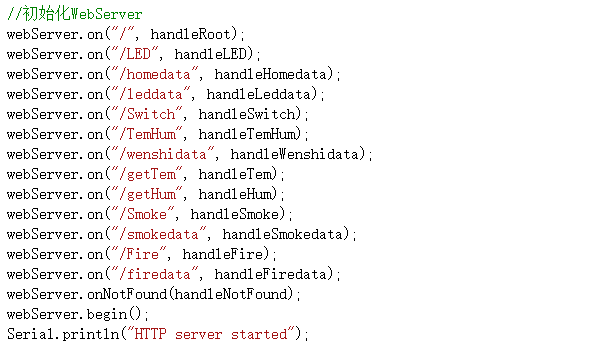
\includegraphics[width=0.8\textwidth]{figures/code/1}
    \caption{初始化WebServer}
\end{figure}

\begin{figure}[htbp]
    \centering
    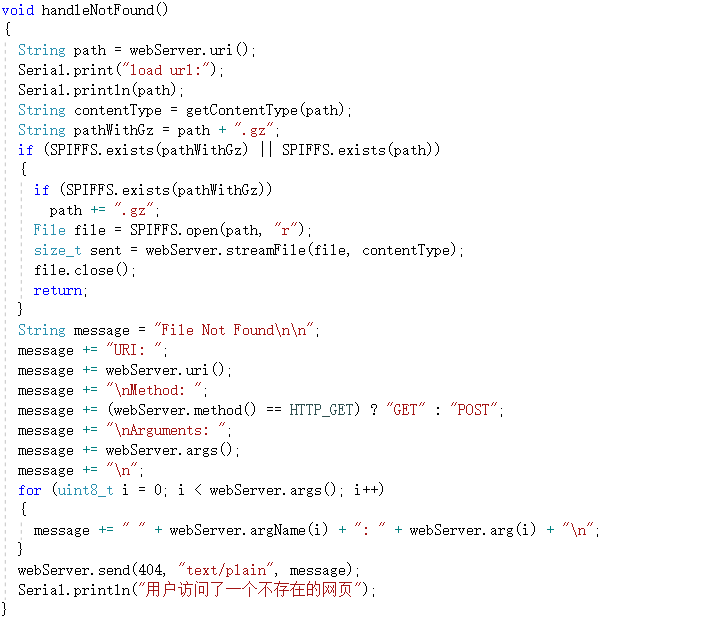
\includegraphics[width=0.8\textwidth]{figures/code/2}
    \caption{handleNotFound()方法}
\end{figure}

\begin{figure}[htbp]
    \centering
    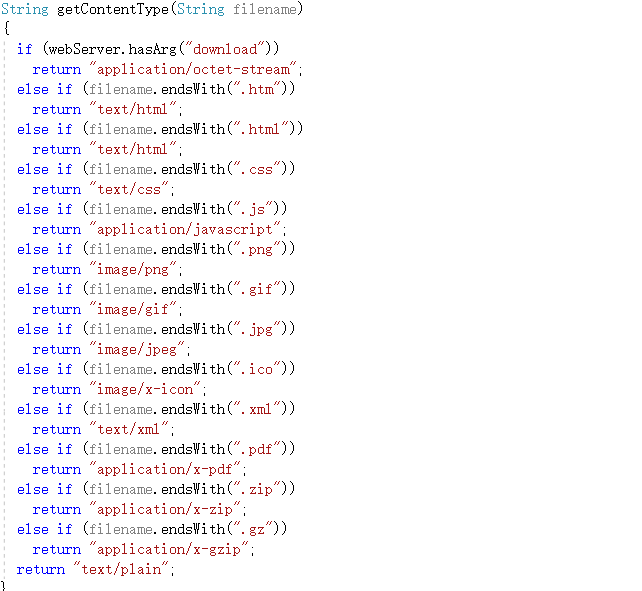
\includegraphics[width=0.8\textwidth]{figures/code/3}
    \caption{getContentType()方法}
\end{figure}

\section{APP界面设计及数据通信}

\begin{enumerate}

\item {APP UI界面设计}:

通过Android Studio的LinearLayout基础框架设计主界面,使用了2个TextView,2个EditText以及一个Button制作TCP连接登陆框架;使用了2个Button制作ESP8266上连接小灯的开关控制;使用了4个TextView制作温湿度以及烟霾数据的时时数据显示窗口;使用了Spinner(下拉菜单)制作查看温湿度历史数据折线图,烟霾历史数据折线图等界面的自由跳转功能。

两个历史数据折线图界面均使用LinearLayout基础框架设计,包含一个TextView显示主题,一个HelloChart的LineChartView绘制折线图,其中HelloChart为Android Studio制作折线图,柱状图等图表的开源库。

\item {APP界面通过Spinner控件自由跳转实现}:

Spinner控件通过Adapter以及Click监听实现Activity之间的切换,通过辨别点击不同的item来跳转相应界面,并使用Intent和Bundle来进行数据的传递,以保证历史数据的存储方便绘制历史折线图。由于Spinner控件最初若连续点击相同item不会进行响应只会对有别于之前选中的选项进行事件响应,所以使用AdapterView中的事件绑定的方式更改相同事件可重复进行的变量,实现点击相同item仍进行跳转。

\begin{figure}[htbp]
    \centering
    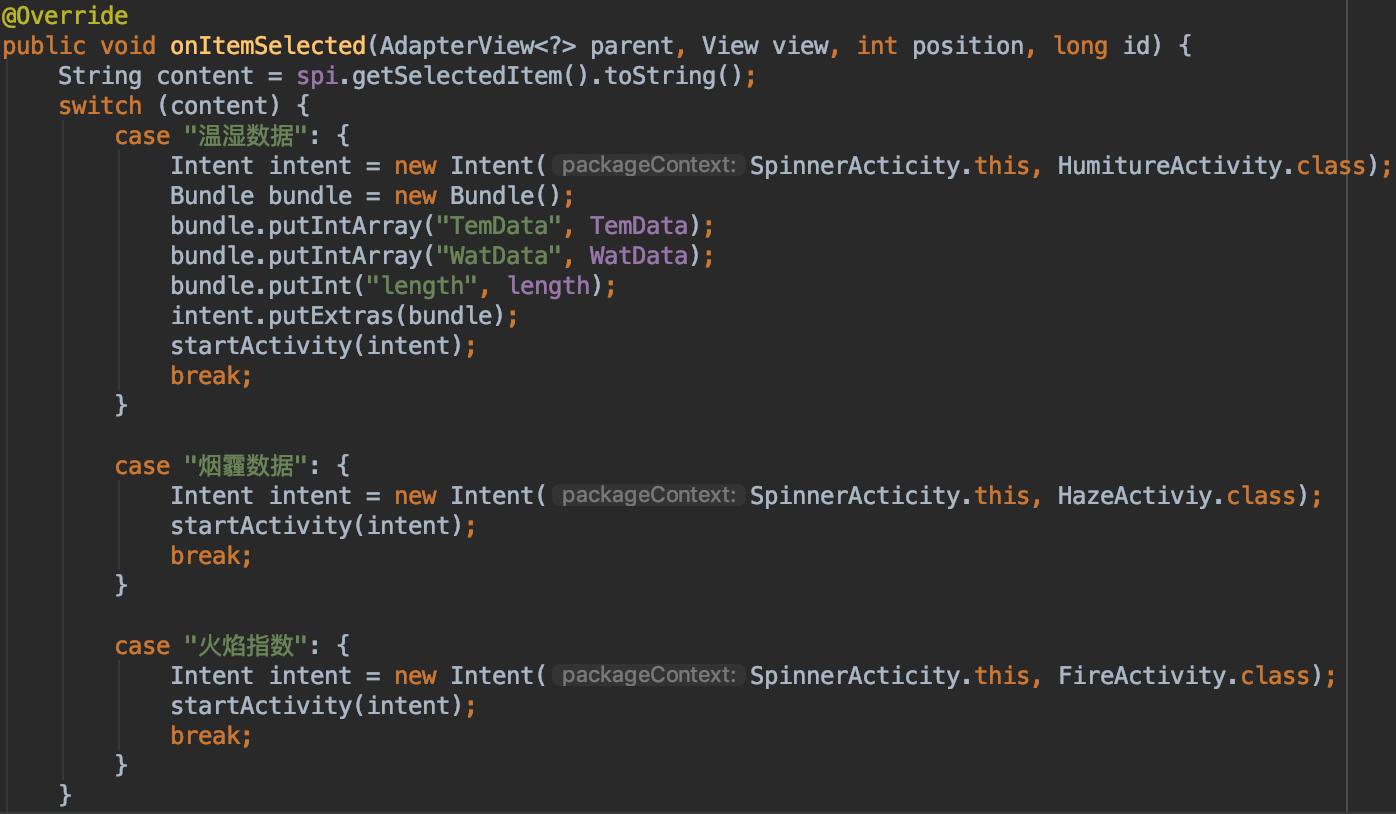
\includegraphics[width=0.8\textwidth]{figures/code/6}
    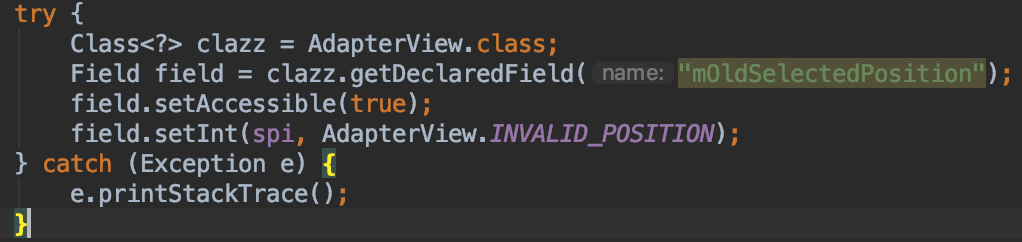
\includegraphics[width=0.8\textwidth]{figures/code/7}
    \caption{页面跳转}
\end{figure}

\item {APP与ESP8266建立TCP连接以及数据传输接受实现}:

通过监听连接Button的点击情况,使用线程以及socket传输与局域网服务器建立连接,ESP8266方面通过WIFI模块进行相同局域网连接,建立与APP之间的通讯。

\begin{figure}[htbp]
    \centering
    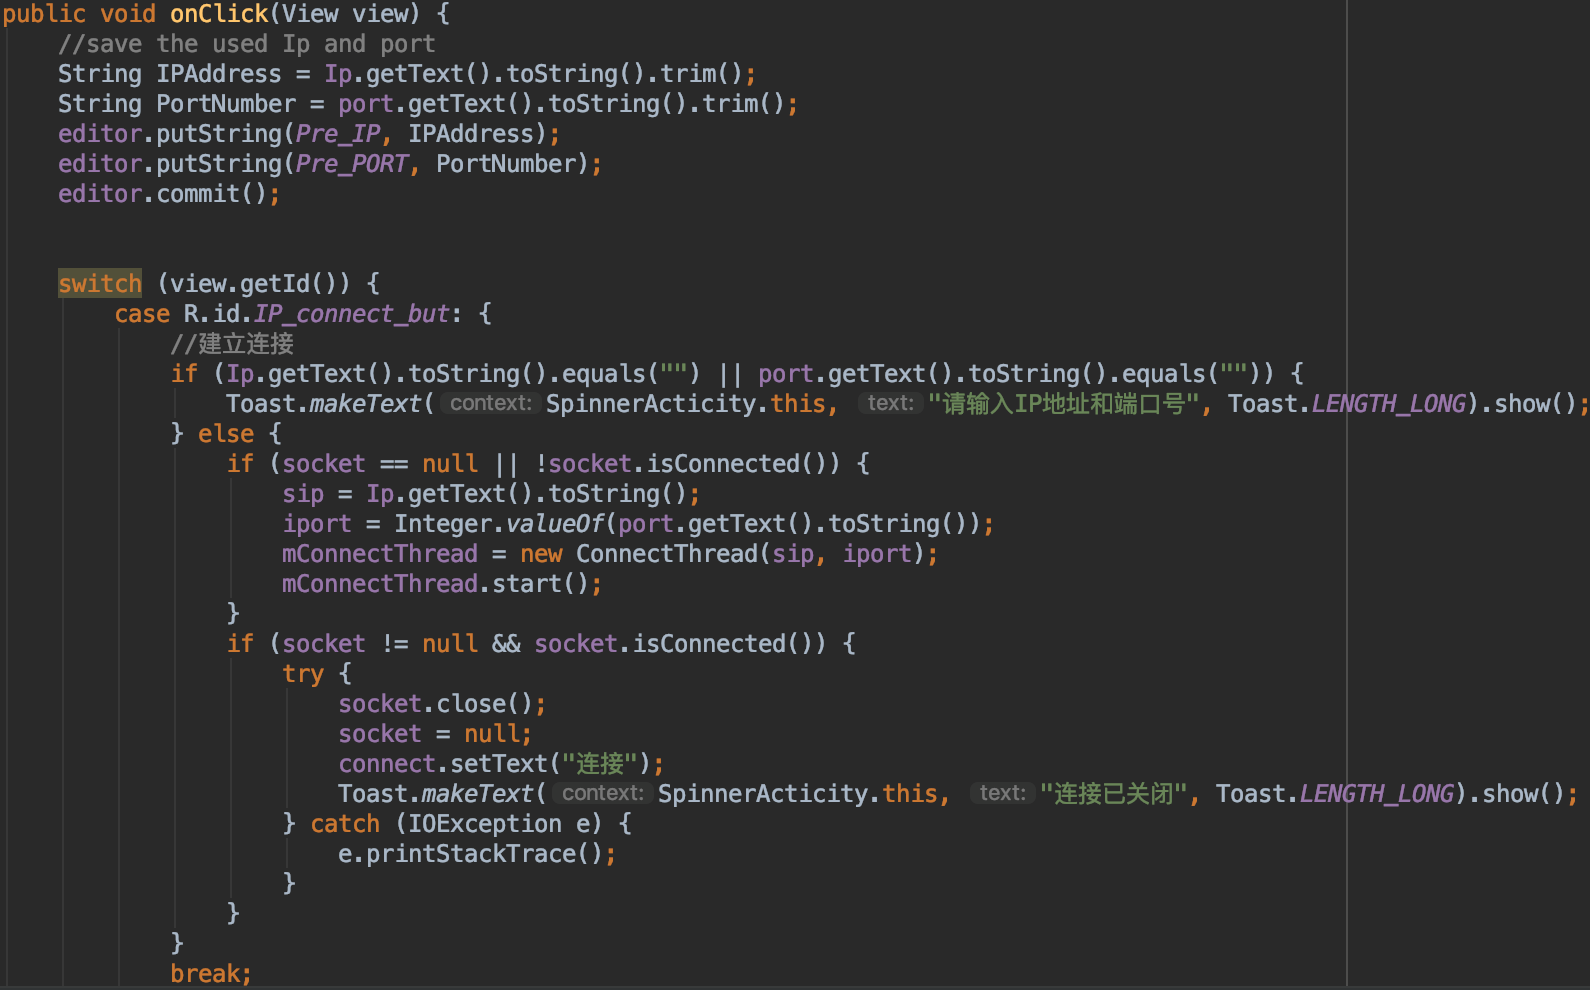
\includegraphics[width=0.8\textwidth]{figures/code/8}
    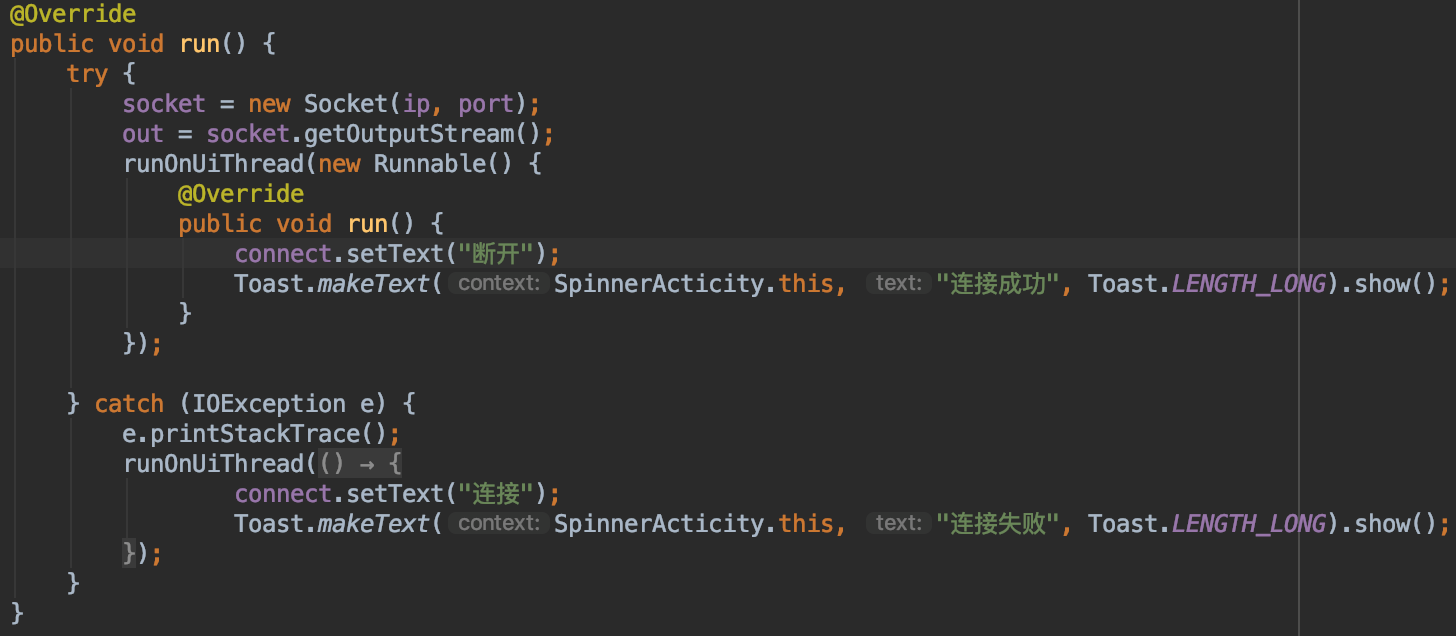
\includegraphics[width=0.8\textwidth]{figures/code/9}
    \caption{TCP协议通信}
\end{figure}

值得注意的是为防止切换界面后导致已输入的IP地址以及端口号清空,连接别打断,特使用了SharedPreferences.Editor来保存记录其连接情况。

传输数据使用的方法是socket的getOutputStream.write,可向服务器发送数据,并在服务器端接收响应回复相应动作,如开关灯即通过按钮监听动作向服务器发送请求数据。

\begin{figure}[htbp]
    \centering
    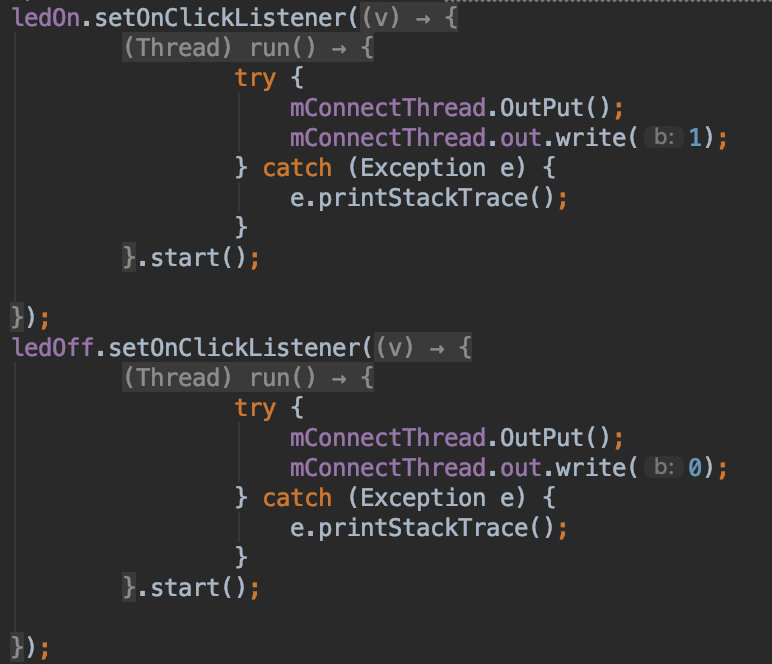
\includegraphics[width=0.8\textwidth]{figures/code/10}
    \caption{监听器}
\end{figure}

接受数据使用方式为客户端app向服务器发送请求数据,服务器返回数据给客户端,客户端调用接受线程ReceiveThread进行解析并接受存储,因温湿度时刻在改变所以使用timer计时器每隔一段时间请求一次数据进行更新。(此步与小组成员石琦合作完成)

\begin{figure}[htbp]
    \centering
    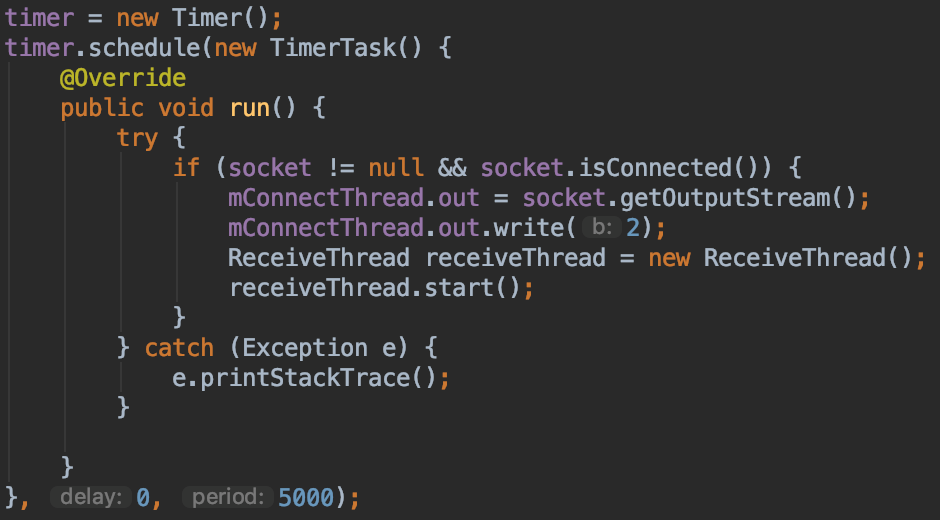
\includegraphics[width=0.8\textwidth]{figures/code/11}
    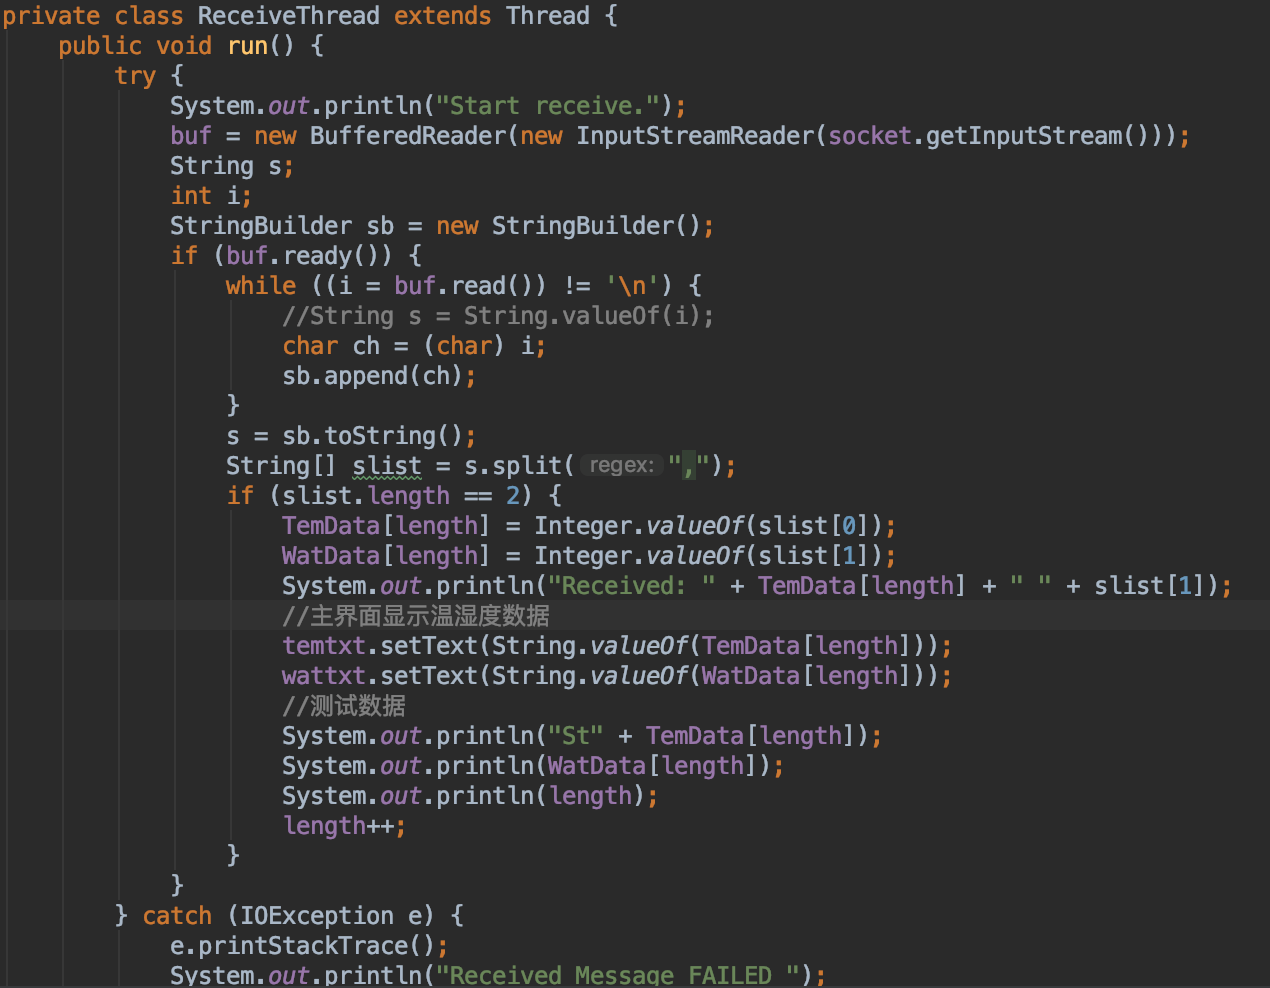
\includegraphics[width=0.8\textwidth]{figures/code/12}
    \caption{计时器和线程ReceiveThread}
\end{figure}

\item {历史数据折线图的绘制}:

首先设置数组通过Bundle和getIntent接受主界面传输回的数据,然后通过HelloChart中的组件先设置数据点的集合,然后设置两条不同的线分别代表不同数据传入到线集合中。

\begin{figure}[htbp]
    \centering
    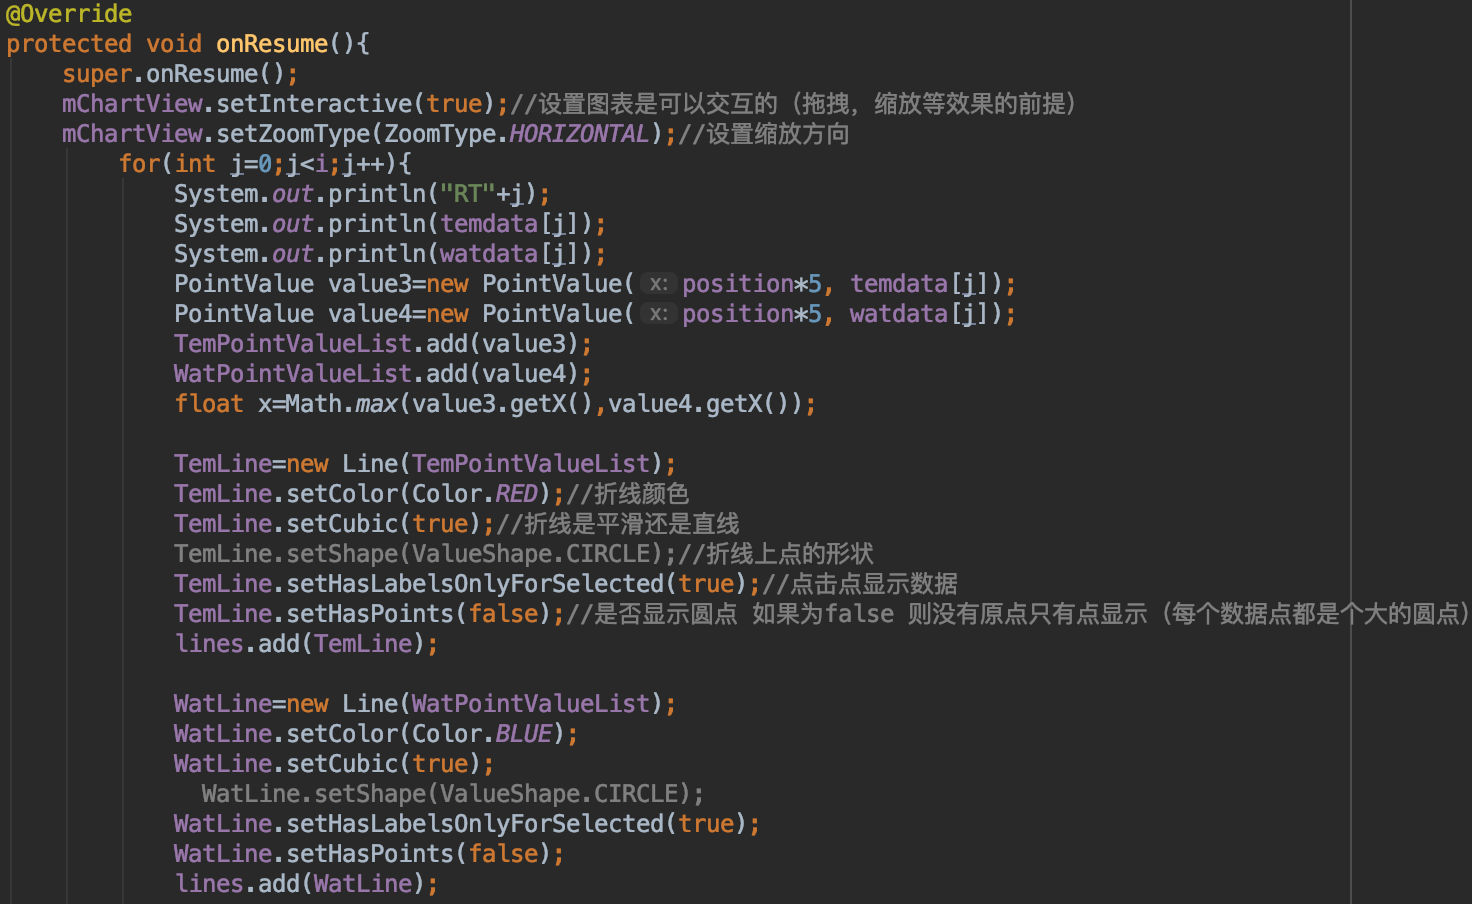
\includegraphics[width=0.8\textwidth]{figures/code/13}
\end{figure}

使用函数initData建立坐标轴X,Y,并建立函数设置坐标图的最大数据显示范围以及当前数据显示区域。可根据当前数据情况进行折线图的动态移动,为折线图设置属性setInteractive以及setZoomType可以对折线图进行拖动查看。

\begin{figure}[htbp]
    \centering
    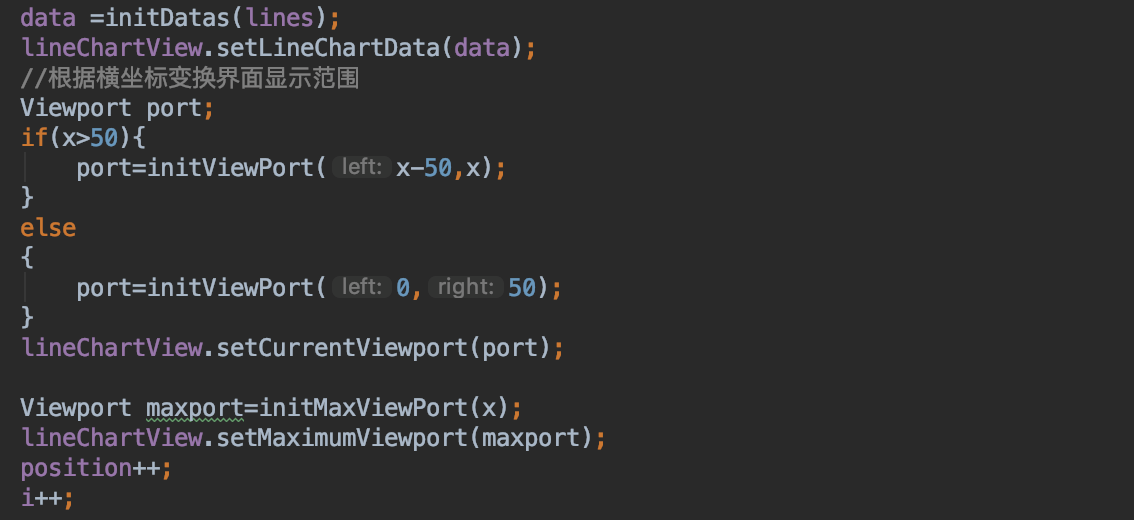
\includegraphics[width=0.8\textwidth]{figures/code/14}
    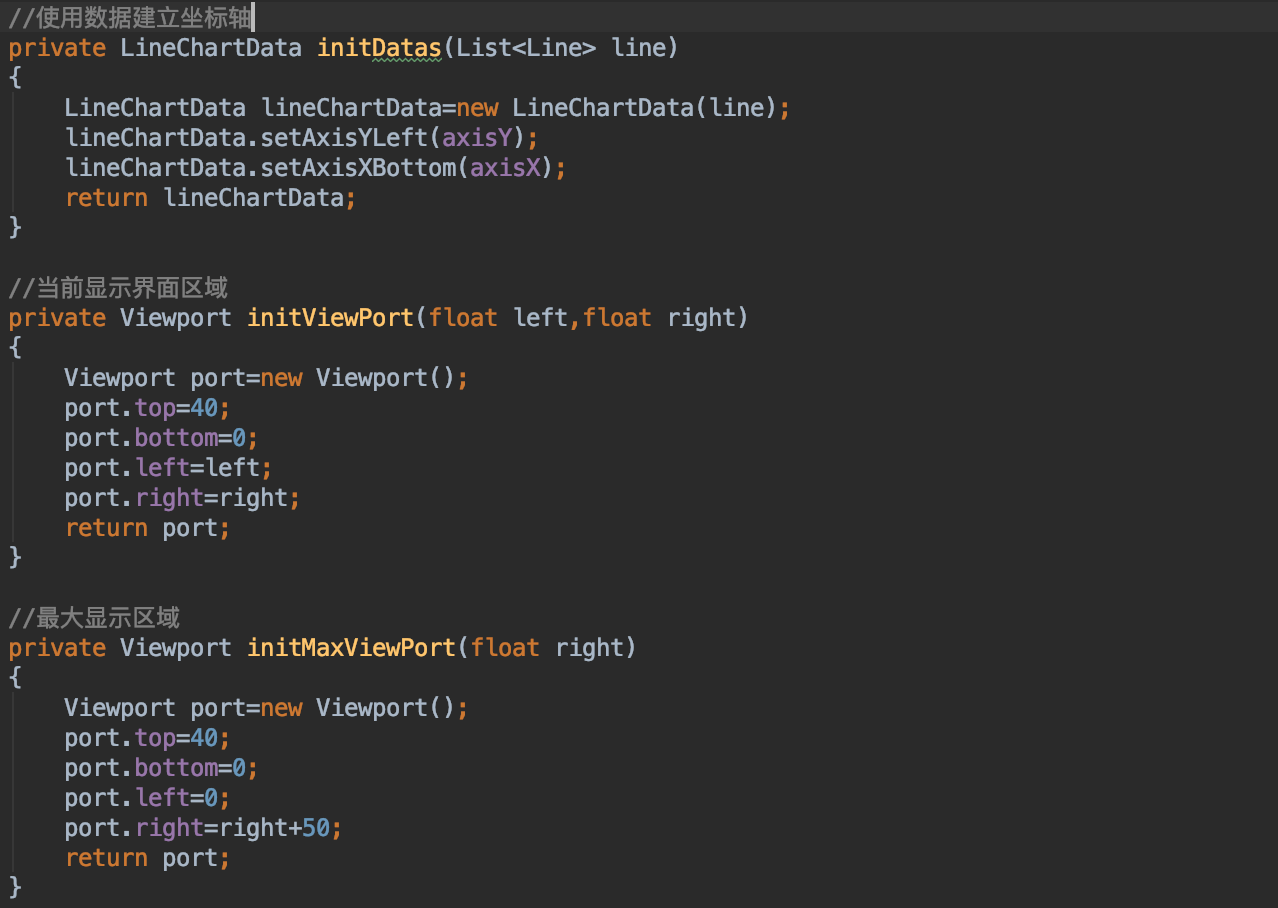
\includegraphics[width=0.8\textwidth]{figures/code/15}
\end{figure}

函数PrintHumitureLine进行对坐标轴X,Y的属性设置以及折线图行为属性的设置,开始使用数据进行进行绘图。

\begin{figure}[htbp]
    \centering
    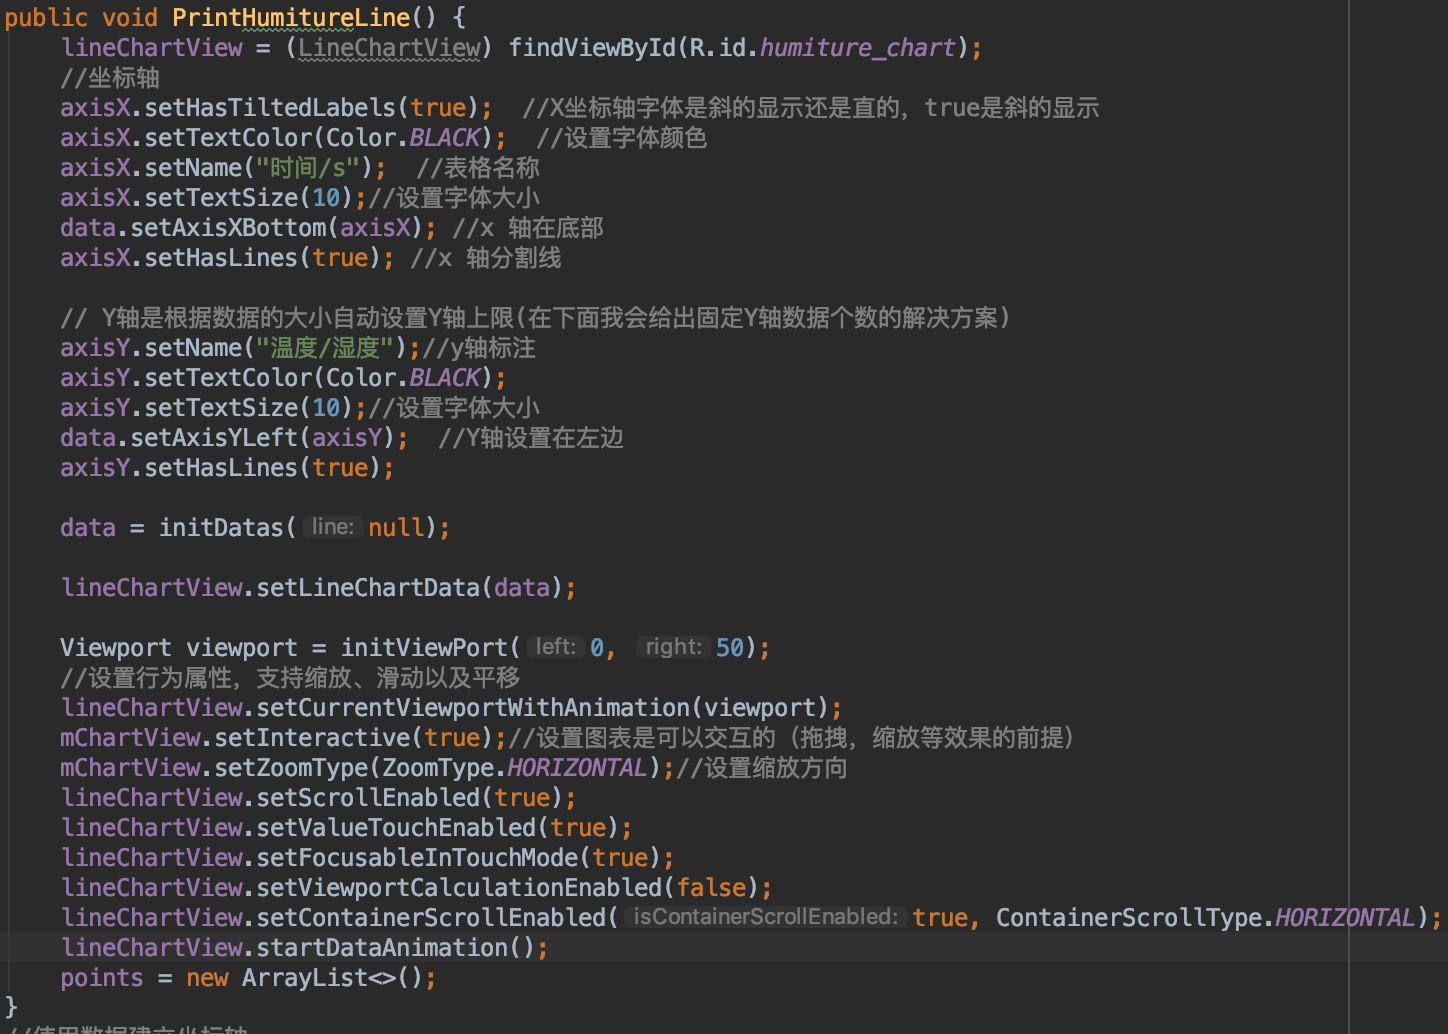
\includegraphics[width=0.8\textwidth]{figures/code/16}
\end{figure}

\end{enumerate}

\section{Web页面设计及数据通信}

考虑到需求的功能主要有控制LED灯的开关、检测室内温湿度、检测烟雾、检测火焰四个方面,并且与APP相照应,故而将网页设计为主页、LED灯、温湿数据、烟霾数据、火焰指数五个页面,并为五个页面设计导航栏。

在主页中,添加一个slider用来动态显示几个传感器的图片,增加页面美感。同时在下方显示所有数据并实时自动更新。自动刷新数据使用setInterval(function, time)定时调用。获取数据使用XMLHttpRequest()方法,并在单片机中烧录相关响应代码,即使用webServer.on()方法接收请求,用webServer.send()方法发送响应,主要代码如下:

\begin{figure}[htbp]
    \centering
    
\includegraphics[width=0.8\textwidth]{figures/code/4}
    \caption{使用XMLHttpRequest()方法与服务器通信}
\end{figure}

LED页面实时监听LED灯的开关状态,并随之改变img的src属性,使之实现开关灯的图片效果,仍然使用http的方式与服务区通信。

温湿数据页面同样用定时器实时显示室内温湿度数据,除此之外,还使用jQuery+Highcharts包绘制温湿度历史数据折线图,每五秒刷新一次数据,增加一条折线。实现代码如下:

\begin{figure}[htbp]
    \centering
    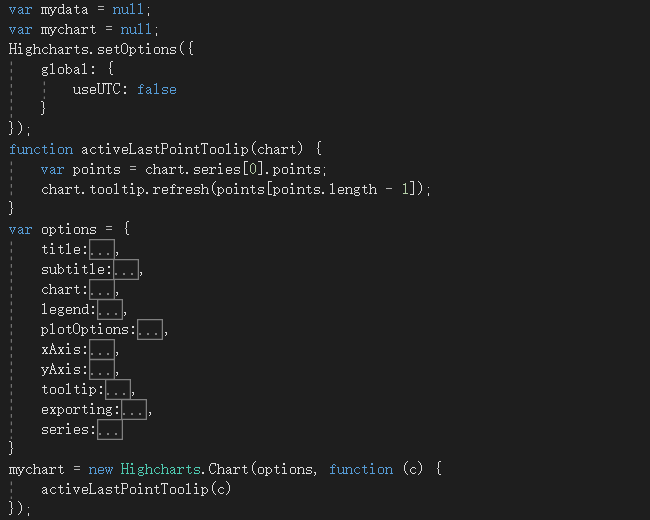
\includegraphics[width=0.8\textwidth]{figures/code/5}
    \caption{Highcharts折线图的属性}
\end{figure}

烟霾指数页面和火焰指数页面用定时器实时刷新服务器端的烟雾数据和火焰情况,并在出现火焰的时候在火焰指数界面使用alert()弹出警告提示框。